\documentclass[a4paper]{article}
\usepackage[utf8x]{inputenc}
\usepackage[T1,T2A]{fontenc}
\usepackage[russian]{babel}
\usepackage{hyperref}
\usepackage{indentfirst}
\usepackage{listings}
\usepackage{color}
\usepackage{here}
\usepackage{array}
\usepackage{multirow}
\usepackage{graphicx}

\usepackage{caption}
\renewcommand{\lstlistingname}{Программа} % заголовок листингов кода

\usepackage{listings}
\lstset{ %
extendedchars=\true,
keepspaces=true,
language=bash,					% choose the language of the code
basicstyle=\footnotesize,		% the size of the fonts that are used for the code
numbers=left,					% where to put the line-numbers
numberstyle=\footnotesize,		% the size of the fonts that are used for the line-numbers
stepnumber=1,					% the step between two line-numbers. If it is 1 each line will be numbered
numbersep=5pt,					% how far the line-numbers are from the code
backgroundcolor=\color{white},	% choose the background color. You must add \usepackage{color}
showspaces=false				% show spaces adding particular underscores
showstringspaces=false,			% underline spaces within strings
showtabs=false,					% show tabs within strings adding particular underscores
frame=single,           		% adds a frame around the code
tabsize=2,						% sets default tabsize to 2 spaces
captionpos=b,					% sets the caption-position to bottom
breaklines=true,				% sets automatic line breaking
breakatwhitespace=false,		% sets if automatic breaks should only happen at whitespace
escapeinside={\%*}{*)},			% if you want to add a comment within your code
postbreak=\raisebox{0ex}[0ex][0ex]{\ensuremath{\color{red}\hookrightarrow\space}}
}

\usepackage[left=2cm,right=2cm,
top=2cm,bottom=2cm,bindingoffset=0cm]{geometry}


\begin{document}	% начало документа

\begin{titlepage}	% начало титульной страницы

	\begin{center}		% выравнивание по центру

		\large Санкт-Петербургский Политехнический Университет Петра Великого\\
		\large Институт компьютерных наук и технологий \\
		\large Кафедра компьютерных систем и программных технологий\\[6cm]
		% название института, затем отступ 6см
		
		\huge Программирование\\[0.5cm] % название работы, затем отступ 0,5см
		\large Отчет по курсовой работе\\[0.1cm]
		\large Игра tower defence\\[5cm]

	\end{center}


	\begin{flushright} % выравнивание по правому краю
		\begin{minipage}{0.25\textwidth} % врезка в половину ширины текста
			\begin{flushleft} % выровнять её содержимое по левому краю

				\large\textbf{Работу выполнил:}\\
				\large Курякин Д. А.\\
				\large {Группа:} 23501/4\\
				
				\large \textbf{Преподаватель:}\\
				\large Вылегжанина К.Д.

			\end{flushleft}
		\end{minipage}
	\end{flushright}
	
	\vfill % заполнить всё доступное ниже пространство

	\begin{center}
	\large Санкт-Петербург\\
	\large \the\year % вывести дату
	\end{center} % закончить выравнивание по центру

\thispagestyle{empty} % не нумеровать страницу
\end{titlepage} % конец титульной страницы

\vfill % заполнить всё доступное ниже пространство



% Содержание
\tableofcontents
\newpage



\section{Игра tower defense}

\subsection{Игровые принадлежности}

Tower Defense сокращенно TD — название жанра компьютерных стратегических игр. Задача игрока в играх подобного жанра — расправиться с наступающими врагами, называемыми «крипы» до того, как они пересекут карту, с помощью строительства башен, атакующих их, когда те проходят вблизи. Противники и башни различаются по характеристикам и цене. Когда враги побеждены, игрок зарабатывает очки, которые используются для покупки или модернизации башен. Подбор башен и их расположение — неотъемлемая стратегия игры. Ползучие твари пробегают через подобие лабиринта, что дает игроку возможность стратегического размещения башен.

\subsection{Порядок использования}

Пользователь ставит башенки на поле, затем нажимает на кнопку готовности, начинается появление крипов. 

\section{Проектирование приложения}

\subsection{Концепция приложения} 

В ходе проектирования было разработана концепция продукта.
Созданное приложение должно предполагать возможность добавление и удаление башен с поля, появление крипов с последующим уничтожение базы и отстрел крипов башнями.

\subsection{Минимально работоспособный продукт}

Минимальном работоспособным продуктом было признано приложение, позволяющие производить игру. 

\subsection{Прецеденты использования}

На основе разработанной концепции была составлена UML диаграмма прецедентов использования (рис.\ref{pic:use_case}).

\begin{figure}[H]
	\begin{center}
		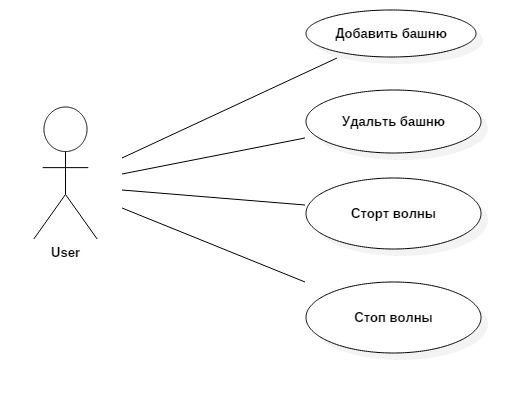
\includegraphics[width=1\textwidth]{../image/use_case.png}
		\caption{Диаграмма прецедентов использования}
		\label{pic:use_case}
	\end{center}
\end{figure}

\subsection{Основные компоненты приложения}

На основе анализа концепции и выделенных прецедентов использования было принято решение выделить два основных компонента, которые будут входить в состав продукта:

\begin{enumerate}
	\item Библиотека
	
	 Включает в себя игровую модель и реализует игровые механизмы. В ядре должно быть обеспечено регулярное обновление модели в ответ на действие пользователя. Кроме того, должна быть реализована обработка исключительных ситуаций, включающие в себя ошибки игрока, попытки выполнить запрещенные действия и прочее.
	
	\item Графическое приложение 

	Графически визуализирует игровую модель, предоставляет пользователю графический интерфейс для взаимодействия с ней и выполнения остальный действий предусмотренных в реализации библиотеки. 
\end{enumerate}

\subsection{Используемые инструменты}

Разработка в основном велась с использованием средств стандартной библиотеки Java в среде IntelliJ IDEA. Для создания графического интерфейса применялась библиотека Swing. 

\subsubsection{IntelliJ IDEA}

IntelliJ IDEA — интегрированная среда разработки программного обеспечения на многих языках программирования, в частности Go, Java, JavaScript, Python, разработанная компанией JetBrains.

\subsubsection{Swing}

Swing — библиотека для создания графического интерфейса для программ на языке Java. Swing был разработан компанией Sun Microsystems. Он содержит ряд графических компонентов, таких как кнопки, поля ввода, таблицы и т. д.

Swing относится к библиотеке классов JFC, которая представляет собой набор библиотек для разработки графических оболочек. К этим библиотекам относятся Java 2D, Accessibility-API, Drag \& Drop-API и AWT.

\subsection{Выводы}
Таким образом, была разработана концепция приложения, что позволило определить внешний вид продукта и выделить его основные компоненты.

\section{Реализация приложения}

\subsection{Среда разработки}

\begin{itemize}
\item Операционная система: Windows 10
\item Интегрирование среда разработки: IntelliJ IDEA 2016.2.3
\item Система автоматической сборки: Gradle 2.14
\item Компилятор: javac, JDK 8.101
\end{itemize}

\subsection{Реализация основных компонентов приложения}

\subsubsection{Библиотека Core}
	
	Для реализации всех запланированных функциональностей было принято решение, создать пятнадцать классов:
	
	\begin{enumerate}
		
	\item \textbf{Класс Enemy}
	Данный класс представляет возможность создания списка противников. Конструктор класса \textbf{Enemy} получает на вход индекс противника \textbf{id}, урон \textbf{damage}, жизни \textbf{health}и скорость \textbf{speed}. И добавляет противника в список.
	
	\item \textbf{Класс EnemySlime}
	Наследуется от класса \textbf{Enemy}. Создаёт противника slime.
	
	\item \textbf{Класс EnemyBigSlime}
	Наследуется от класса \textbf{Enemy}. Создаёт противника большой slime.	
	
	\item \textbf{Класс EnemyMove} 
	
	Данный класс хранит в себе координаты каждого противника. 
	
	Конструктор класса \textbf{EnemyMove} получает на вход ссылку на противника и координаты появления.
	
	\item \textbf{Класс Base}
	Хранит в себе координаты базы на карте.
	
	\item \textbf{Класс EnemyRoute}
	Конструктор класса \textbf{EnemyRoute} получает на вход индекс противника данные с карты и ищет координаты появления противника на карте с помощью класса \textbf{SpawnPoint}, добавляет координаты к себе в список. Метод \textbf{calculateRoute} с помощью метода \textbf{calculateNextPos} прощитывает путь от места появления противников до базы игрока.
	
	 \item \textbf{Класс EnemyAIMove} 
	 Перемещает выбранного противника по карте используя метод \textbf{move}. Метод \textbf{move} используя класс \textbf{EnemyRoute} передвигает противников.
	 
	\item \textbf{Класс EnemyAI} 
	Конструктор класса \textbf{EnemyAI} с помощью класса \textbf{EnemyRoute} ищет дорогу и добавляет к себе в поле класса.
	
	\item \textbf{Класс Tower} 
	Данный класс представляет возможность создания списка башен. Конструктор класса \textbf{Tower} получает на вход индекс башни \textbf{id}, стоимость \textbf{cost}, радиус поражения \textbf{range}, урон \textbf{damage}. И добавляет башню в список.
	
	\item \textbf{Класс TowerFire}
	Наследуется от класса \textbf{Tower}. Создаёт огненную башню.
	
	\item \textbf{Класс TowerLightning}
	Наследуется от класса \textbf{Tower}. Создаёт электрическую башню.
	
	\item \textbf{Класс TowerMap}
	Конструктор класса \textbf{TowerMap} создаёт матрицу размером 14 на 14 типа \textbf{Tower}. Метод \textbf{AddTower} принимает на вход координаты башни \textbf{x, y} и индекс башни \textbf{id} затем добавляет башню на поле вычитая стоимость постройки башни из класса \textbf{User}. Метод \textbf{DeleteTower} принимает на вход координаты башни \textbf{x, y} затем удаляет башню с поля прибавляя процент от стоимости башни в класса \textbf{User}.
	
	\item \textbf{Класс User}
	Хранит в себе монеты и жизни игрока и проверяет. С помощью метода \textbf{gameOver} проверяет есть ли у базы игрока жизни если нет то игра окончена. 
	
	\item \textbf{Класс Map}
	С помощью класса \textbf{LevelFile} считывает данные о уровне с файла и добавляет к себе. С помощью класса \textbf{Level} ищет координаты появления противника.
	
	\item \textbf{Класс Wave}
	С помощью метода \textbf{spawnEnemies} создает волны противников.
	
	\end{enumerate}
	
\subsubsection{Графический интерфейс}

Для создания графического интерфейса использовалась библиотека Java Swing. 
С помощью Qt Widgets было созданы классыд двух основных окон \textbf{Interface} и \textbf{FieldGUI}, которые отвечали за основное меню и вывод сотки кроссворда. 

\begin{figure}[H]
	\begin{center}
		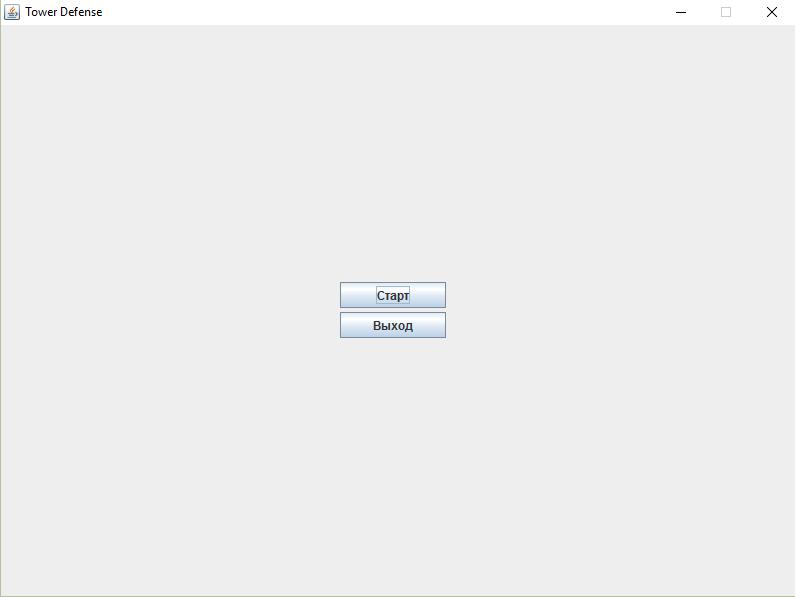
\includegraphics[width=1\textwidth]{../image/menu.png}
		\caption{Меню графического интерфейса}
		\label{pic:gui_menu}
	\end{center}
\end{figure} 

\begin{figure}[H]
	\begin{center}
		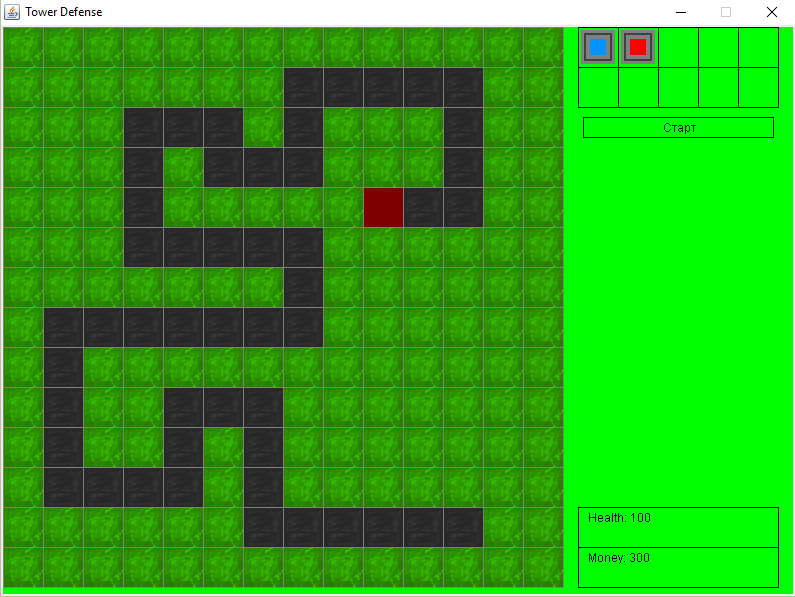
\includegraphics[width=1\textwidth]{../image/GameScreen1.png}
		\caption{Игровое окно графического интерфейса}
		\label{pic:gui_screen1}
	\end{center}
\end{figure} 

\begin{figure}[H]
	\begin{center}
		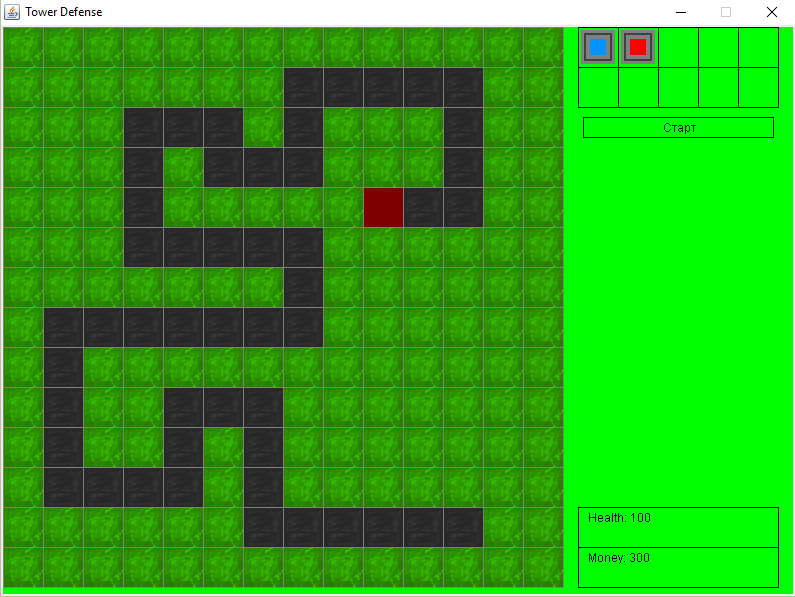
\includegraphics[width=1\textwidth]{../image/GameScreen1.png}
		\caption{Игровое окно графического интерфейса}
		\label{pic:gui_screen2}
	\end{center}
\end{figure} 



На рисунках \ref{pic:gui_menu}, \ref{pic:gui_screen1} и \ref{pic:gui_screen2} изображены основные окна графического приложения. 

\subsection{Теститрование}

В ходе разработки проекта регулярно проводилось ручное тестирование.

Тестирование позволило обеспечить работоспособность продукта в ходе всего процесса разработки. 

\subsection{Демонстрации}

Во время создания приложения было проведено 1 демонстрации, на которых группой людей, представляющих собой потенциальных пользовоталей разработываемого приложения, были сделаны различные замечания и высказаны множество предложений и пожеланий, основанных на внешнем виде продукта и стандартном цикле работы с ним. Анализ полученной информации позволял обнаруживать недочеты присутсвующие в продукте на том, или ином этапе разработки, а также определять дальнейшие направления улучшения и расширения проекта, что, безусловно, положительно сказалось на конечном результате.

\section{Выводы}

В ходе работы были получены навыки необходимые для написания программ на языке программирования Java. Во-первых была изучена стандартная библиотека, библиотека Swing и особенности данного языка. Во-вторых был получен опыт, связанный с процессом разработки программного продукта. 

\section{Приложение 1}

\subsection{Листинги}



\end{document}